%! TeX program = xelatex

\documentclass[12pt, a4paper]{article}
\usepackage{cmap}
\usepackage[fontsize=12pt]{scrextend}
\usepackage[T2A]{fontenc}
\usepackage[utf8]{inputenc}
\usepackage[english,russian]{babel}
\usepackage{amsmath,amsfonts,amssymb,amsthm,mathtools}
\usepackage[left=20mm, top=20mm, right=20mm, bottom=20mm, nohead, footskip=1cm]{geometry}
\usepackage{multirow}
\usepackage{array}
\usepackage{multicol}
\usepackage{graphicx}
\usepackage{wrapfig}
\usepackage{indentfirst}
\usepackage{enumitem}

\usepackage{polyglossia}
\usepackage{titlesec}
\usepackage{sectsty}
\usepackage{setspace}
\usepackage{fontspec}
\defaultfontfeatures{Mapping=tex-text}

\usepackage{lipsum}
\usepackage{tocloft}
\usepackage[dvipsnames]{xcolor}

\usepackage{caption}
%\captionsetup{labelfont=it, textfont=it}
%\captionsetup[figure]{name=Схема}

\usepackage{hyperref}

\hypersetup{
    colorlinks=false,
    linktoc=all
}
\urlstyle{same}

\setmainlanguage{english}
\setotherlanguage{russian}
\setkeys{russian}{babelshorthands=true}
\setmainfont{Times New Roman}
\newfontfamily\cyrillicfont{Times New Roman}
%\let\cyrillicfonttt\ttfamily
%\onehalfspacing

%\allsectionsfont{\centering}
\renewcommand{\cftsecleader}{\cftdotfill{\cftdotsep}}

%======================================SECTIONING=========================================
%\makeatletter
%\renewcommand*\l@section{\@dottedtocline{1}{1.5em}{2.3em}}
%\makeatother
%======================================SECTIONING=========================================

\pretolerance=6000
\tolerance=3000
\emergencystretch=4pt

\setlength\intextsep{10pt}

\graphicspath{{./visuals/}}
\setlength{\parskip}{0.3125cm}
\setlength{\parindent}{1.25cm}
\setlength{\columnsep}{1cm}
\author{Grigoryev Mikhail}
\title{Algs lab}

\begin{document}

\thispagestyle{empty}

\vspace{30mm}

\begin{center}
FEDERAL STATE AUTONOMOUS EDUCATIONAL INSTITUTION \\
OF HIGHER EDUCATION \\
ITMO UNIVERSITY

\vspace{40mm}

{\large \textbf{Report \\
on the practical task No. 5 \\
"Algorithms on graphs. Introduction to graphs and basic algorithms on graphs"}}
\end{center}

\vspace{15mm}

\begin{flushright}
{\large Performed by \\
\textit{Mikhail Grigoryev (370852) \\
Semenova Valeria (370061) \\
Academic group J4133c \\}
Accepted by \\
Dr Petr Chunaev}
\end{flushright}

\vspace{80mm}

\begin{center}
St. Petersburg \\
2022
\end{center}

\newpage

\section*{Goal}
\addcontentsline{toc}{section}{Goal}

The use of different representations of graphs and basic algorithms on graphs (Depth-first search and Breadth-first search).

\section*{Formulation of the problem}
\addcontentsline{toc}{section}{Formulation of the problem}

\textbf{Task 1.} Generate a random adjacency matrix for a simple undirected unweighted graph of 100 vertices and 200 edges (note that the matrix should be symmetric and contain only 0s and 1s as elements). Transfer the matrix into an adjacency list. Visualize the graph and print several rows of the adjacency matrix and the adjacency list. Which purposes is each representation more convenient for?

\textbf{Task 2.} Use Depth-first search to find connected components of the graph and Breadth-first search to find a shortest path between two random vertices. Analyse the results obtained.

\section*{Brief theoretical part}
\addcontentsline{toc}{section}{Brief theoretical part}

Path search algorithms on graphs are used to find shortest paths between two vertices. In case of unweighted graphs, those paths consist of the least number of edges.

Algorithms used in this practical work (implemented from NetworkX library):
\begin{enumerate}
	\item Depth-first search (here for finding connected components) was implemented from scratch recursively. DFS utilizes a neighbor stack (unlinke BFS which uses a queue). It is a simple algorithm that looks at all neighbors of the current vertex, puts them on the stack, then takes the first neighbor in the stack and that vertex becomes current. This results in the vertices in one branch being traversed first.
	\item Breadth-first search (here for finding the shortest path) was taken from NetworkX. The method \textit{nx.shortest\_path} was used, if the graph is unweighted, BFS is used by default. It is a traversal algorithm similar to DFS. However, BFS uses a neighbor queue, thus the vertices closest to the stariting one are being traversed first.
\end{enumerate}

\newpage

\section*{Results}
\addcontentsline{toc}{section}{Results}

\textbf{Task 1.} A random adjacency matrix of a simple undirected graph $G(|V|=100, |E|=200)$ was generated. The matrix is symmetrical (undirected graph) and contains only 1s (edge) and 0s (no edge). The first 3 rows of the adjacency matrix were printed.

\noindent
First row: {\footnotesize [0. 0. 0. 0. 0. 0. 0. 0. 0. 0. 0. 0. 0. 0. 0. 0. 0. 1. 0. 0. 0. 0. 0. 0. 0. 0. 0. 0. 0. 0. 0. 0. 0. 0. 0. 0. 0. 0. 0. 0. 0. 0. 0. 0. 0. 0. 0. 0. 0. 0. 0. 1. 0. 0. 0. 0. 0. 0. 0. 0. 0. 0. 0. 1. 0. 0. 0. 0. 0. 0. 0. 1. 0. 0. 0. 0. 0. 0. 0. 0. 0. 0. 0. 0. 0. 0. 0. 0. 0. 0. 0. 0. 0. 0. 0. 0. 0. 0. 1. 0.]}

\noindent
Second row: {\footnotesize [0. 0. 0. 0. 0. 0. 0. 0. 0. 0. 0. 0. 0. 0. 0. 0. 0. 0. 0. 0. 0. 0. 0. 0. 0. 0. 0. 0. 0. 0. 0. 0. 0. 0. 0. 0. 0. 0. 1. 0. 0. 0. 0. 0. 0. 0. 0. 0. 0. 0. 0. 0. 0. 0. 0. 0. 0. 0. 0. 0. 0. 0. 0. 0. 0. 0. 0. 0. 0. 0. 0. 0. 0. 0. 0. 0. 0. 0. 1. 0. 0. 0. 0. 0. 0. 0. 0. 0. 0. 0. 0. 0. 0. 0. 0. 0. 0. 0. 0. 0.]}

\noindent
Third row: {\footnotesize [0. 0. 0. 0. 0. 0. 0. 0. 0. 0. 0. 0. 0. 0. 0. 0. 0. 0. 0. 0. 0. 0. 0. 0. 0. 0. 0. 0. 0. 0. 0. 0. 0. 0. 0. 0. 0. 0. 0. 0. 0. 1. 0. 0. 0. 0. 0. 0. 1. 0. 0. 0. 0. 0. 0. 0. 0. 0. 0. 0. 0. 0. 1. 0. 0. 0. 0. 0. 0. 0. 1. 0. 0. 0. 0. 0. 0. 0. 0. 0. 0. 0. 0. 0. 0. 0. 0. 0. 0. 0. 0. 0. 0. 0. 0. 0. 0. 0. 0. 0.]}

The adjacency matrix was transferred to an adjacency list which is either a list (or a dictionary) of lists of neighbors. The first 3 rows are presented below:

\noindent
First row: {\footnotesize [17, 51, 63, 71, 98]}

\noindent
Second row: {\footnotesize [38, 78]}

\noindent
Third row: {\footnotesize [41, 48, 62, 70]}

Additionally, the graph was visualized.
\begin{figure}[!h]
\centering
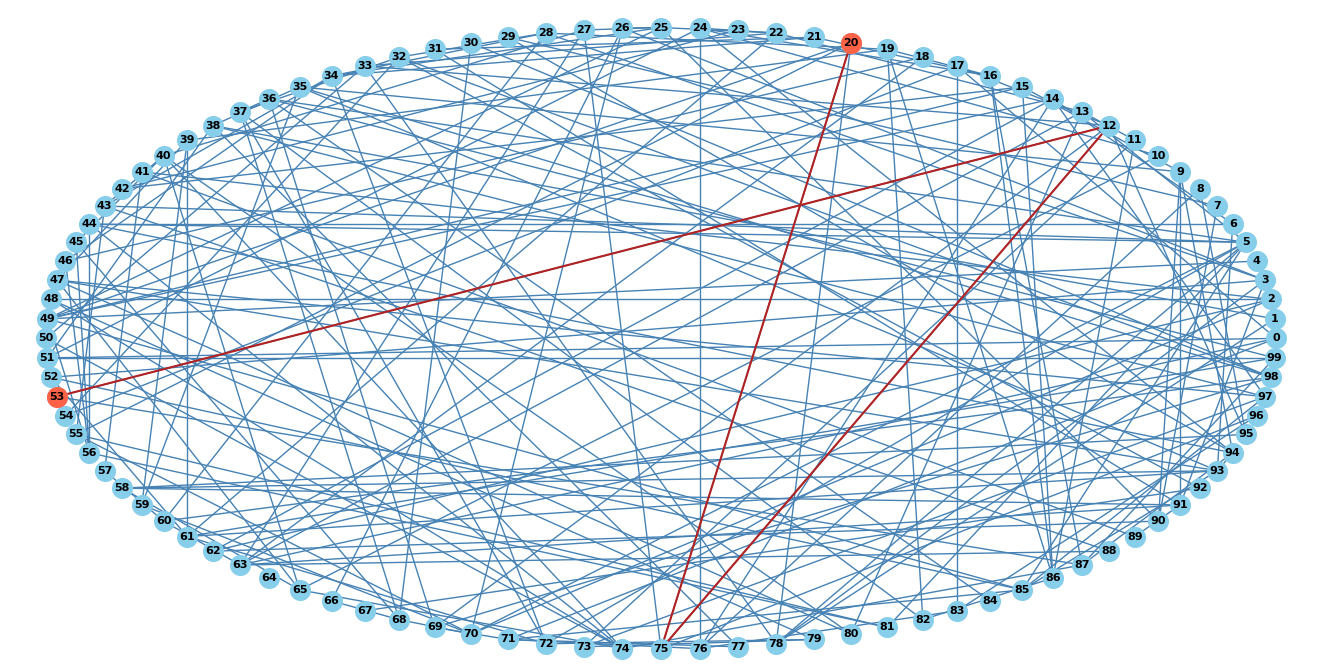
\includegraphics[width=0.9\textwidth]{graph.png}
\caption{The random undirected graph with 100 vertices and 200 edges visualized (with shortest path between two random vertices).}
\end{figure}

The printed rows show that adjacency lists are significantly more space-efficient than adjacency matrices. Additionally, they are more legible for humans as we can read the rows of the adjacency list as: \textit{the 0th vertex is adjacent to vertices 17, 51, 63, 71 and 98}. Both of the structures are better representations than plain visuals that get complicated even for small graphs.

\newpage

\textbf{Task 2.} In the second task, DFS was used to find connected components of the generated graph. For the graph visualized previously, the connected components were: vertex number 64 and all the other vertices (they happened to be connected). The code in the listing (see Appendix) prints both connected components and all connected vertices (in pairs).

BFS was used to compute the shortest path between a pair of random vertices (from 53 to 20). The path for the mentioned vertices was:
\[ 53 \to 12 \to 75 \to 20 \]
The path contains 3 edges and 4 vertices. This path was visualized previously. The algorithm provides a path for any pair of vertices, if they are connected.

\section*{Conclusions}
\addcontentsline{toc}{section}{Conclusions}

Different representations of graphs were compared. Graph traversal algorithms for unweighted graphs such as Depth- and Breadth-first search were applied for searching the shortest path between random vertices in random graphs and for yielding connected components of the graph.

\section*{Appendix}
\addcontentsline{toc}{section}{Appendix}

GitHub link: \url{https://github.com/Dormant512/itmo_lab_listings/blob/main/lab5.py}.

\begin{figure}[!h]
\centering

\includegraphics[width=0.25\textwidth]{lab5.png}
\end{figure}


\end{document}
